% Select one class
%\documentclass{pucthesis}		% For DVI
\documentclass[pdftex]{pucthesis}	% For pdfLaTeX
%\documentclass[spanish]{pucthesis}		% For DVI, in spanish
%\documentclass[pdftex,spanish]{pucthesis}	% For pdfLaTeX, in spanish

%%%%%%%%%%%%%%%%%%%%%%%%%%
%      Nota: si usas español, algunos nombres      %
%      debes cambiarlos manualmente en este     %
%        documento. En teoría, nunca deberías       %
%           modificar el archivo pucthesis.cls              %
%%%%%%%%%%%%%%%%%%%%%%%%%%

%%%%%%%%%
%   Packages	 %
%%%%%%%%%

% Floats
\usepackage{graphicx}
\usepackage{float}
\floatstyle{boxed}
\restylefloat{figure}
\usepackage{subfigure}
\usepackage{color}

% Math packages
\usepackage{amsmath}
\usepackage{amsfonts}
\usepackage{amssymb}

% Closest font to Times New Roman
\usepackage{times}

% To make pretty tables
\usepackage{booktabs}
\usepackage{multirow}

% To avoid underfull errors in the bibliography
\usepackage{etoolbox}
\apptocmd{\sloppy}{\hbadness 10000\relax}{}{}

% To make cites and references
\usepackage[hidelinks,pdfusetitle,pdfdisplaydoctitle]{hyperref}
\usepackage[notocbib]{apacite} 
\usepackage{doi}
\renewcommand{\doitext}{}

%--------- NEW ENVIRONMENTS --------- You are free to remove or use it
\newtheorem{definition}{\bf Definition}[chapter]
\newtheorem{property}{Property}[chapter]
\newtheorem{claim}{Claim}[chapter]
\newtheorem{lemma}{\bf Lemma}[chapter]
\newtheorem{proposition}{Proposition}[chapter]
\newtheorem{theorem}{\noindent \bf Theorem}[chapter]
\newtheorem{corollary}{\bf Corollary}[chapter]
\newtheorem{pf}{Proof}[chapter]
\newtheorem{example}{\bf Example}[chapter]
\newtheorem{remark}{Remark}[chapter]

\makeatletter
  \setlength{\beftitle}{105\p@\@plus24\p@}
  \setlength{\afttitle}{65\p@}
\makeatother

\begin{document}

\mdate{Month Day, Year}         % date manuscript changed
\version{1}                                     % manuscript version #

\title[(LONG THESIS TITLE)]
   {\bf (LONG  THESIS TITLE)}       
\author[Author's Name]{Author's name}

\address{Escuela de Ingenier\'ia\\
                   Pontificia Universidad Cat\'olica de Chile\\ 
                   Vicu\~na Mackenna 4860\\
                  Santiago, Chile\\
                  {\it Tel.\/} : 56 (2) 354-2000}
\email{username@uc.cl}

\facultyto    {the School of Engineering}
%\department   {}
\faculty                             {Faculty of Engineering}
\degree                  {Master of Science in Engineering}  %   {Mag\'ister en Ciencias de la Ingenier\'ia}  %        
                                 % or {Doctor in Engineering Sciences}    % {Doctor en Ciencias de la Ingenier\'ia}
\advisor                            {Professor's name}
\committeememberA {Member A}
\guestmemberA            {Member B}
\ogrsmember                 {Member C}
\subject                            {Structural Engineering}
\date                                 {Month Year}
\copyrightname             {Author's name}
\copyrightyear               {MMXV}
\dedication                      {Gratefully to my parents and siblings}

%%%%%%%%%%%%%%%%%%%%
%       PRELIMINARIES                              %
%----------------------------------------------------%
%      page i & ii: cover page                   %
%      page iii: dedication                         %
%%%%%%%%%%%%%%%%%%%%

\NoChapterPageNumber
\pagenumbering{roman}
\maketitle

%%%%%%%%%%%%%%%%%%%%
%   EXTRA PAGES                                     %
%----------------------------------------------------%
%      page --: not used                             %
%%%%%%%%%%%%%%%%%%%%

%\newpage
%\thispagestyle{empty}

%----------------------------------------------------------------------%

%%%%%%%%%%%%%%%%%%%%%%%%%
%      page v: ACKNOWLEDGEMENTS                   %
%%%%%%%%%%%%%%%%%%%%%%%%%

\phantomsection \label{acknowledgements} % Comment if hyperref is unused
\chapter*{ACKNOWLEDGEMENTS}           
Thanks to my family and girlfriend for their unmeasurable support during the time
this research was done. Thanks to my advisor for his great guidance and contributions.
Thanks to all the members of \textit{IALAB PUC} and \textit{Instituto Milenio Fundamentos de los Datos}
project \#4 for all the very useful feedback and conversations. Thanks to ANID (former CONICYT) for
granting me the National Masters scholarship, which enabled me to complete my studies without
any issues.





\cleardoublepage

%----------------------------------------------------------------------%

%%%%%%%%%%%%%%%%%%
%          page v & up ---                      %
%            Table of contents              %
%            List of figures                     %
%            List of tables                      %
%%%%%%%%%%%%%%%%%%

\pdfbookmark{\contentsname}{toc}
\tableofcontents
\phantomsection \label{listoffigures}
\listoffigures
\phantomsection \label{listoftables}
\listoftables
\cleardoublepage

%----------------------------------------------------------------------%

%%%%%%%%%%%%%%%%%%%%%%%%
%      page x & xi: ABSTRACT - RESUMEN        %
%%%%%%%%%%%%%%%%%%%%%%%%

\phantomsection \label{abstract}
\chapter*{ABSTRACT}
Urban perception has been an important research subject for at least 60 years, with studies
being conducted by many different disciplines, using a variety of methodologies mainly based
on surveys over either real or simulated urban environments. The recently increased availability
of large amounts of data and highly scalable data collection methods powered by the modern web
has allowed for new techniques from other domains to be extended to the estimation of urban perception.
In particular, machine learning methods used as either stand alone models or feature extraction tools
have proven to be very effective for automatic quantification of the perception. This methods (neural networks in particular) present the disadvantage of having a black box
nature, which can make it hard for humans to understand the obtained results, therefore limiting
their application.

In this work we present a novel neural network architecture for automatic urban perception quantification.
Our best model, named AttnSegRank, can output an estimated urban perception score based on an image,
along with a set of weights (displayable as a heatmap) that reflect the importance of each part of the image
on the calculation of the score. It achieves this by including the output of a pretrained
semantic segmentator leveraged with an attention mechanism as part of the architecture. The model
we show in this work presents very similar performance with those in the previous literature but
with a much better interpretability, making it  not only a more useful model for urban perception
measuring and research, but a contribution to explainability in
the deep learning and computer vision fields that can be applied to other tasks as well.


\vfill
\noindent {\bf Keywords}:  urban perception, deep learning, explainable artificial intelligence.

\cleardoublepage

\phantomsection \label{resumen}
\chapter*{RESUMEN}
El resumen debe contener entre 100 y 300 palabras. El resumen debe ser escrito en ingl\'es y espa\~nol.  En el caso de tesis de doctorado, el formato de la p\'agina del resumen es distinta, por favor verifique la plantilla entregada por la Direcci\'on de Postrgrado.\

\vfill
\noindent {\bf Palabras Claves}: percepción urbana, aprendizaje profundo, inteligencia artificial explicable.

\cleardoublepage

%%%%%%%%%%%%%
%   TEXT  OF THESIS     %
%%%%%%%%%%%%%

\pagenumbering{arabic}

\chapter[INTRODUCTION]{Introduction}
\section{Thesis outline.}
\section{Importance of automatic urban perception}
\section{Importance of explainability in artificial intelligence}
\section{Hypothesis}

\chapter[CHAPTER 1]{Chapter 1} \label{ch1}
\input{./chapters/chapter1.tex}

\chapter[CHAPTER 2]{Chapter 2} \label{ch2}
\input{./chapters/chapter2.tex}

\chapter[CONCLUSIONS]{Conclusions}
Nothing to say. Be happy.

\section{Contribution to the state of the art}

%%%%%%%%%%%%%
%       REFERENCES        %
%%%%%%%%%%%%%

\cleardoublepage
\phantomsection \label{references}
\bibliographystyle{apacite}
\renewcommand{\bibname}{REFERENCES}

%%%% ACTIVAR SIGUIENTES 3 LINEAS SI POSTGRADO RECHAZA LA BIBLIOGRAFIA
%\setlength{\bibleftmargin}{0em}
%\setlength{\bibindent}{0em}
%\setlength{\bibitemsep}{1em}


\bibliography{Thesis}

%%%%%%%%%%%%
%      APPENDICES      %
%%%%%%%%%%%%

\appendix % It is like a chapter, so each appendix (A, B, C...) must to be considered as a section

\newpage
\section[First Appendix]{First Appendix}
\subsection{Visual representation}
\label{sec:seg_colors}
For visually representing segmentation, we make a color map over the images, following
the cityscapes color palette \cite{cordts_cityscapes}. See figure \ref{fig:segmentation_colors}
for the exact palette and class list, and figure \ref{fig:cs_sample} for an example.

\begin{figure}[ht]
	\begin{center}
	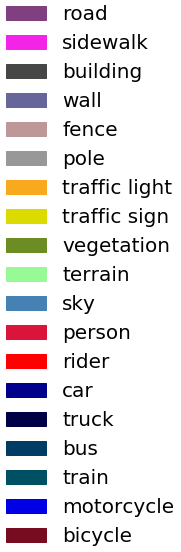
\includegraphics[width=0.2\textwidth]{./figures/seg_colors.png}
	\caption[Segmentation color palette]{
        Segmentation color palette.
        }
	\label{fig:segmentation_colors}
	\end{center}
\end{figure}

\begin{figure}[ht]
	\begin{center}
	\includegraphics[width=1\textwidth]{./figures/cityscapes_sample.png}
	\caption[CityScapes sample]{
        CityScapes sample.
        }
	\label{fig:cs_sample}
	\end{center}
\end{figure}

\subsection{Segmentation distribution}
\label{sec:seg_distribution}
Given the domain shift from Cityscapes to PlacePulse, is important to check how
the segmentation behaves on the new dataset.

The most significant difference between the datasets is the image size, which are almost 13
times bigger in cityscapes, allowing for smaller objects like traffic signs to be clearly
distinguishable. In training CS images are used with size of $769 \times 769$, while
place pulse images are used with the standard $224\times224$. Another important difference
is the origin of the images, while Cityscapes images were all taken on different cities of
the same developed country (Germany), PlacePulse images come from 56 cities distributed on all
continents, including both developed and developing countries, with the later ones contributing
images with a significant visual difference.

Table \ref{tab:segmentation} show the percentage of pixels belonging to each segmentation class
on the entire set of images of the PlacePulse dataset. Evidently this are not ground truth labels,
but the ones obtained by our  PspNet trained on Cityscapes. As was expected, classes representing
physically smaller objects have an almost negligible contribution since the smaller image size renders
them pretty much unidentifiable. Domain shift makes the model constantly confuse the sidewalk (which can
be seen in a large percentage of PlacePulse images) with the main road, reducing the class presence
to a very underwhelming 0.96\%. Same behavior can be perceived with the terrain class.


\begin{table}[H]
	\begin{tabular}{|l|r|} \hline
	Segmentation Class & \% of pixels \\ \hline
	Building      & 26.60\% \\
	Vegetation    & 25.52\% \\
	Road          & 24.21\% \\
	Sky           & 6.24\%  \\
	Fence         & 5.09\%  \\
	Truck         & 2.96\%  \\
	Car           & 1.94\%  \\
	Person        & 1.48\%  \\
	Bicycle       & 1.36\%  \\
	Motorcycle    & 1.28\%  \\
	Sidewalk      & 0.96\%  \\
	Wall          & 0.89\%  \\
	Terrain       & 0.65\%  \\
	Pole          & 0.33\%  \\
	Train         & 0.26\%  \\
	Bus           & 0.14\%  \\
	Traffic sign  & 0.05\%  \\
	Traffic light & 0.02\%  \\
	Rider         & 0.02\%  \\ \hline
	\end{tabular}
	\caption[Segmentation Distribution]{
		Pixel distribution of the segmentation classes over the PlacePulse Dataset
	}
	\label{tab:segmentation}
\end{table}

\newpage
\section[An Interesting Short Story]{An Interesting Short Story}
Here we present the full significance tables from the results discussed in section \ref{sec:significance}

\begin{table}[H]
	\begin{tabular}{|l|rrrrrrr|}
		\hline
					& \multicolumn{7}{c|}{\textbf{Significance \%}}   \\ \hline
		\textbf{Class}         & \textbf{Wealthy}        & \textbf{Depressing}     & \textbf{Safety}         & \textbf{Boring}         & \textbf{Lively}         & \textbf{Beautiful}      & \textbf{Average}        \\
		\hline
		Road          & 62.46          & \textbf{77.98} & \textbf{78.64} & 31.77          & \textbf{90.58} & 17.33        & \textbf{59.79} \\
		Building      & \textbf{63.74} & 9.21           & 30.35          & \textbf{82.69} & 17.99          & \textbf{52.79} & 42.80          \\
		Sky           & 43.81          & 44.51          & 39.34          & 18.34          & 45.68          & 45.80          & 39.58          \\
		Person        & 4.86           & 18.18          & 10.83          & 28.83          & 25.76          & 6.77           & 15.87          \\
		Car           & 4.09           & 19.70          & 12.02          & 34.63          & 6.12           & 15.50          & 15.34          \\
		Vegetation    & 4.27           & 22.56          & 20.57          & 5.50           & 5.45           & 24.08          & 13.74          \\
		Bicycle       & 4.81           & 8.25           & 10.32          & 15.48          & 16.57          & 10.10          & 10.92          \\
		Sidewalk      & 10.65          & 12.46          & 2.21           & 7.65           & 7.35           & 9.66           & 8.33           \\
		Truck         & 4.65           & 11.38          & 2.94           & 9.57           & 6.29           & 14.29          & 8.19           \\
		Motorcycle    & 4.92           & 5.31           & 6.68           & 8.10           & 9.77           & 10.97          & 7.63           \\
		Wall          & 3.43           & 4.63           & 4.90           & 9.95           & 5.33           & 9.14           & 6.23           \\
		Fence         & 5.33           & 13.15          & 6.83           & 1.75           & 2.17           & 4.55           & 5.63           \\
		Pole          & 1.48           & 2.76           & 2.04           & 8.00           & 13.03          & 3.49           & 5.13           \\
		Terrain       & 0.74           & 2.72           & 2.72           & 13.31          & 1.45           & 4.38           & 4.22           \\
		Traffic sign  & 1.18           & 2.39           & 1.47           & 3.55           & 2.59           & 1.44           & 2.10           \\
		Traffic light & 1.60           & 0.89           & 0.47           & 2.00           & 1.19           & 1.42           & 1.26           \\
		Train         & 0.22           & 1.57           & 0.16           & 0.73           & 0.52           & 3.84           & 1.17           \\
		Bus           & 0.74           & 1.51           & 1.15           & 0.82           & 0.83           & 0.92           & 1.00           \\
		Rider         & 0.49           & 1.12           & 1.02           & 1.10           & 1.23           & 0.98           & 0.99 \\
		\hline
	\end{tabular}
	\caption[Percentage of class significance]{
		Percentage of images where a segmentation class is considered significant over the entire PlacePulse dataset.
	}
	\label{tab:total_sig}
\end{table}


\begin{table}[H]
	\begin{tabular}{|l|rrrrrrr|}
		\hline
					& \multicolumn{7}{c|}{\textbf{Significance \%}} \\ \hline
		\textbf{Class} & \textbf{Wealthy} & \textbf{Depressing} & \textbf{Safety} & \textbf{Boring} & \textbf{Lively} & \textbf{Beautiful} & \textbf{Average} \\
		\hline
		Sky            & \textbf{78.49}   & \textbf{80.12}      & 70.85           & 33.32           & 82.16           & \textbf{82.62}     & \textbf{71.26}   \\
		Road           & 64.87            & 81.01               & \textbf{81.67}  & 33.06           & \textbf{94.07}  & 18.00              & 62.12            \\
		Rider          & 30.34            & 65.75               & 59.74           & 61.42           & 71.21           & 59.14              & 57.93            \\
		Building       & 69.73            & 10.07               & 33.23           & \textbf{90.59}  & 19.67           & 57.81              & 46.85            \\
		Wall           & 25.11            & 34.35               & 36.34           & 72.00           & 39.70           & 67.03              & 45.75            \\
		Motorcycle     & 23.73            & 25.34               & 32.13           & 38.80           & 46.53           & 51.87              & 36.40            \\
		Bus            & 26.46            & 53.96               & 40.25           & 27.17           & 29.32           & 31.90              & 34.84            \\
		Bicycle        & 14.42            & 24.77               & 30.73           & 45.93           & 49.26           & 30.07              & 32.53            \\
		Person         & 9.61             & 35.91               & 21.37           & 56.87           & 50.77           & 13.35              & 31.31            \\
		Car            & 6.53             & 31.41               & 19.16           & 55.41           & 9.73            & 24.66              & 24.48            \\
		Truck          & 13.13            & 31.95               & 8.26            & 26.92           & 17.51           & 40.09              & 22.98            \\
		Sidewalk       & 28.19            & 33.39               & 5.87            & 20.48           & 19.56           & 25.78              & 22.21            \\
		Traffic sign   & 12.00            & 24.43               & 15.18           & 36.81           & 26.60           & 15.08              & 21.68            \\
		Traffic light  & 26.92            & 15.04               & 8.06            & 34.47           & 20.28           & 24.78              & 21.59            \\
		Train          & 3.96             & 29.40               & 2.95            & 13.57           & 9.38            & 69.82              & 21.52            \\
		Terrain        & 3.35             & 12.39               & 12.40           & 61.04           & 6.63            & 20.23              & 19.34            \\
		Vegetation     & 4.87             & 25.70               & 23.45           & 6.26            & 6.21            & 27.42              & 15.65            \\
		Pole           & 3.89             & 7.19                & 5.35            & 21.04           & 34.17           & 9.15               & 13.46            \\
		Fence          & 10.88            & 26.98               & 14.06           & 3.61            & 4.47            & 9.35               & 11.56            \\
		\hline
	\end{tabular}
	\caption[Percentage of class significance when present]{
		Percentage of times a segmentation class is considered significant when it is present in an image.
	}
	\label{tab:presence_sig}
\end{table}

\end{document}
